\section{Апробация}
\subsection{Тестирование алгоритма}
Тестирование алгоритма композиционального символьного исполнения проводилось на методах, написанных на языке C\#.
Они содержали сложные потоки управления: использовались операторы goto, вложенные циклы, неструктурируемые циклы.
Например, на листинге~\ref{example:fors} показан такой метод.
\begin{lstlisting}[language={[Sharp]C}, caption={Программа, содержащая вложенные циклы},captionpos=b,
label={example:fors}]
public static int NestedFors2(int x)
{
    int sum = 0;
    for (int i = 1; i <= x; i++)
    {
        for (int j = 1; j <= i; j++)
        {
            sum += j;
        }
    }

    return sum;
}
\end{lstlisting}

Его результаты показаны на следующей картинке.
\begin{figure}[H]
\centering
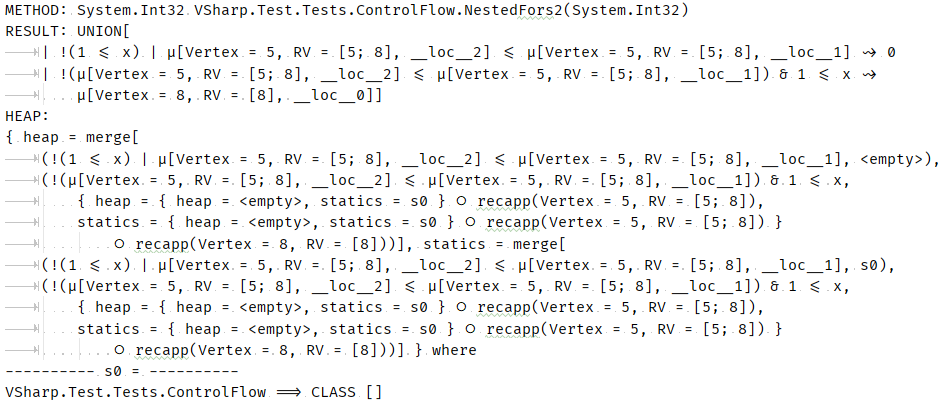
\includegraphics[scale=0.6]{Batoev/images/results.PNG}
\caption{Результат символьного исполнения метода~\ref{example:fors}}
% \label{exec-tree}
\end{figure}

\subsection{Тестирование интерпретатора}
Тестирование нового интерпретатора проводилось на тестовой подсистеме проекта <<VSharp.Test>> и на библиотеке \textsc{Chess.NET}.
Подсистема содержит тестовые наборы, затрагивающие различные конструкции и возможности языка C\#:
арифметику, логические операции,
работу с массивами разных размерностей, генерирование исключений, тесты на классы и структуры, включающие взаимодействие со статическими членами и вызовы виртуальных методов,
тесты с неограниченной рекурсией, тесты с \emph{unsafe}-кодом, тесты со строками. 

Таблица~\ref{experiments} показывает результаты проведенного тестирования. 
В наборах тестах с арифметикой и условными конструкциями была часть тестов с генерацией исключений. 
Поскольку схема обработки исключений для языка CIL не была реализована, то данные тесты были некорректно исполнены.
По той же причине не было проведено тестирования на тестовым наборе <<TryCatch>>, 
основное предназначение которого --- инициирование и перехват исключений.

\begin{table}[H]
    \centering
    \begin{tabular}{ |p{3cm}||p{2cm}|p{2cm}|p{2cm}|  }
        \hline
        \multicolumn{4}{|c|}{Количественные характеристики тестов} \\
        \hline
        Название тестового набора &Количество тестов в наборе&Количество успешно пройденных тестов&Количество инструкций CIL\\
        \hline
        Arithmetics   &80    &77    &1968\\
        Logics        &75    &75    &1458\\
        Conditional   &10    &6     &943\\
        Recursive     &5     &5     &751\\
        Lambdas       &2     &2     &404\\
        Generic       &14    &14    &194\\
        Strings       &15    &15    &219\\
        Unsafe        &16    &16    &312\\
        Typecast      &19    &19    &969\\
        Methods       &10    &10    &238\\
        Lists         &9     &9     &1420\\
        Chess.NET     &1     &1     &2723\\
        \hline
        Всего         &256   &249   &11599\\
        \hline
    \end{tabular}
    \captionof{table}{Результаты тестирования}
    \label{experiments}
\end{table}